%%%%%%%%%%%%%%%%%%%%%%%%%%%%%%%%%%%55%%
\begin{frame} [plain]
  \frametitle{}
  \Background[1]
  \begin{center}
  { {\huge 第一讲:普朗克能量子假说 }}
  \end{center}
  \addtocounter{framenumber}{-1}
\end{frame}
%%%%%%%%%%%%%%%%%%%%%%%%%%%%%%%%%%

\begin{frame} 
  \begin{center}
    \animategraphics[height=2in,loop]{30}{figs/gif/test-}{1}{80} 
    \end{center} 
\end{frame}

\begin{frame}
 \frametitle{多页enumerate}    
    \begin{enumerate}
      \item enumerate1
      \item enumerate2
      \item enumerate2 
      \item enumerate2
    \end{enumerate}
\end{frame}

\begin{frame}
  \frametitle{}    
     \begin{enumerate}
      \setcounter{enumi}{5}
       \item enumerate1
       \item enumerate2
       \item enumerate2 
       \item enumerate2
     \end{enumerate}
 \end{frame}


\begin{frame}
    \frametitle{}
    多行公式
    \begin{multline}
            A=\lim_{n\rightarrow\infty}\Delta x\left(a^{2}+\left(a^{2}+2a\Delta x+\left(\Delta x\right)^{2}\right)\right.\label{eq:reset}\\
            +\left(a^{2}+2\cdot2a\Delta x+2^{2}\left(\Delta x\right)^{2}\right)\\
            +\left(a^{2}+2\cdot3a\Delta x+3^{2}\left(\Delta x\right)^{2}\right)\\
            +\ldots\\
            \left.+\left(a^{2}+2\cdot(n-1)a\Delta x+(n-1)^{2}\left(\Delta x\right)^{2}\right)\right)\\
            =\frac{1}{3}\left(b^{3}-a^{3}\right)
    \end{multline}\\
    \begin{align}
      E=m&c^2 & &E=mc^2\\
      E=~&mc^2 & E&=mc^2 \notag \\
      E&=mc^2 & E=~&mc^2\\
      &E=mc^2 & E=m&c^2
\end{align}
\end{frame}

\begin{frame}
  \frametitle{自定义求解}
  \例[1]{求解如下方程
      \[x^2+y^2=z^2\]}
  \解	\\
  \EXP[2]{求解如下方程
  \[x^2+y^2=z^2\]}
  \Solution \\

  \Tips \\
  \Note \\
  \证 \\
\end{frame}

\begin{frame}
  \frametitle{自定义tcbb}
  \tcbb[0.5]{标题}{内容}
  \tcbb{标题}{内容}
\end{frame}

\begin{frame}
  \frametitle{Awesome 字体表}
  \alert{\faHeartbeat, \faStar, \faThumbTack, \faThumbsUp,\faUniversity, \faCircle}
\end{frame}

\begin{frame}
  \frametitle{引用别人的话}
  \begin{quotation}
    "There is nothing new to be discovered in physics now. All that remains is
    more and more precise measurements"   \\
    \rightline{$\cdots$ Lord Kelvin (1900)\hspace{3em}}
\end{quotation}
\end{frame}

\begin{frame}
  \frametitle{公式加框 boxed}
  \framebox[\width]{我是一段话}
  \begin{equation}
    \boxed{\rho(\nu, T) d \nu=\frac{8 \pi}{c^{3}} \frac{h \nu^{3}}{e^{h \nu / K T}-1} d \nu}
  \end{equation}

\end{frame}

\begin{frame}
  \frametitle{内容加框boxedminipage}
  \begin{boxedminipage}{0.9\linewidth}
   % \vspace{-15pt}
    \[\begin{aligned}
    & \text{若}X_i\sim N(\mu_i,\sigma_i^2)\, i=1,2,\cdots,\text{且它们相互独立,则其线性组合:}\\
    & c_0+c_1X_1+c_2X_2+\cdots+c_nX_n\sim N(\mu,\sigma^2)\\
    & \text{其中}c_1,c_2,\cdots,c_n \text{是不全为0的常数,两个参数为:}\\
    & \mu=c_0+c_1\mu_1+\cdots+c_n\mu_n,\qquad \sigma^2=c_1^2\sigma_1^2+c_2^2\sigma_2^2+\cdots+c_n^2\sigma_n^2
    \end{aligned}\]
    \vspace{2pt}
    \end{boxedminipage}
\end{frame}

\begin{frame}{Font feature test}
  \begin{itemize}
    \item Regular
    \item \textit{Italic}
    \item \textsc{Small Caps}
    \item \textbf{Bold}
    \item \textbf{\textit{Bold Italic}}
    \item \textbf{\textsc{Bold Small Caps}}
    \item \texttt{Monospace}
    \item \texttt{\textit{Monospace Italic}}
    \item \texttt{\textbf{Monospace Bold}}
    \item \texttt{\textbf{\textit{Monospace Bold Italic}}}
  \end{itemize}
\end{frame}

\begin{frame}{Columns and Lists}
  \begin{columns}[T,onlytextwidth]
    \column{0.33\textwidth}
      Items
      \begin{itemize}
        \item Milk \item Eggs \item Potatoes
      \end{itemize}

    \column{0.33\textwidth}
      Enumerations
      \begin{enumerate}
        \item First, \item Second and \item Last.
      \end{enumerate}

    \column{0.33\textwidth}
      Descriptions
      \begin{description}
        \item[PowerPoint] Meeh. \item[Beamer] Yeeeha.
      \end{description}
  \end{columns}
\end{frame}

\begin{frame}{Tables}
  \begin{table}
    \caption{Largest cities in the world (source: Wikipedia)}
    \begin{tabular}{@{} lr @{}}
      \toprule
      City & Population\\
      \midrule
      Mexico City & 20,116,842\\
      Shanghai & 19,210,000\\
      Peking & 15,796,450\\
      Istanbul & 14,160,467\\
      \bottomrule
    \end{tabular}
  \end{table}
\end{frame}

\begin{frame}{Math}
  \begin{equation*}
    e = \lim_{n\to \infty} \left(1 + \frac{1}{n} \right)^n
  \end{equation*}
\end{frame}

\begin{frame}{Blocks}
  Three different block environments are pre-defined and may be styled with an
  optional background color.

  \begin{columns}[T,onlytextwidth]
    \column{0.48\textwidth}
      \begin{block}{Default}
        Block content.
      \end{block}

      \begin{alertblock}{Alert}
        Block content.
      \end{alertblock}

      \begin{exampleblock}{Example}
        Block content.
      \end{exampleblock}

    \column{0.48\textwidth}

      %\metroset{block=fill}

      \begin{block}{Default}
        Block content.
      \end{block}

      \begin{alertblock}{Alert}
        Block content.
      \end{alertblock}

      \begin{exampleblock}{Example}
        Block content.
      \end{exampleblock}

  \end{columns}
\end{frame}

\begin{frame}{tikz for Figures}
  \begin{figure}
    \newcounter{density}
    \setcounter{density}{20}
    \begin{tikzpicture}
      \def\couleur{alerted text.fg}
      \path[coordinate] (0,0)  coordinate(A)
                  ++( 90:5cm) coordinate(B)
                  ++(0:5cm) coordinate(C)
                  ++(-90:5cm) coordinate(D);
      \draw[fill=\couleur!\thedensity] (A) -- (B) -- (C) --(D) -- cycle;
      \foreach \x in {1,...,40}{%
          \pgfmathsetcounter{density}{\thedensity+20}
          \setcounter{density}{\thedensity}
          \path[coordinate] coordinate(X) at (A){};
          \path[coordinate] (A) -- (B) coordinate[pos=.10](A)
                              -- (C) coordinate[pos=.10](B)
                              -- (D) coordinate[pos=.10](C)
                              -- (X) coordinate[pos=.10](D);
          \draw[fill=\couleur!\thedensity] (A)--(B)--(C)-- (D) -- cycle;
      }
    \end{tikzpicture}
    \caption{Rotated square from
    \href{http://www.texample.net/tikz/examples/rotated-polygons/}{texample.net}.}
  \end{figure}
\end{frame}

\begin{frame}{Line plots}
  \begin{figure}
    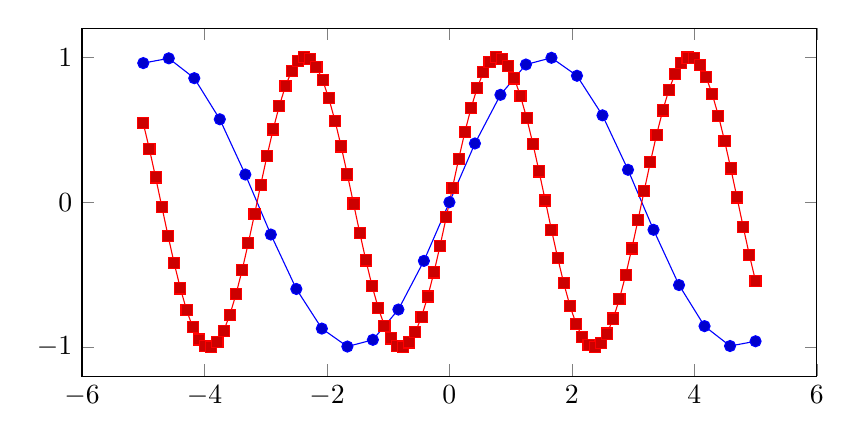
\begin{tikzpicture}
      \begin{axis}[
        width=0.9\textwidth,
        height=6cm,
      ]

        \addplot {sin(deg(x))};
        \addplot+[samples=100] {sin(deg(2*x))};

      \end{axis}
    \end{tikzpicture}
  \end{figure}
\end{frame}


\begin{frame}{3D plots}
\begin{figure}
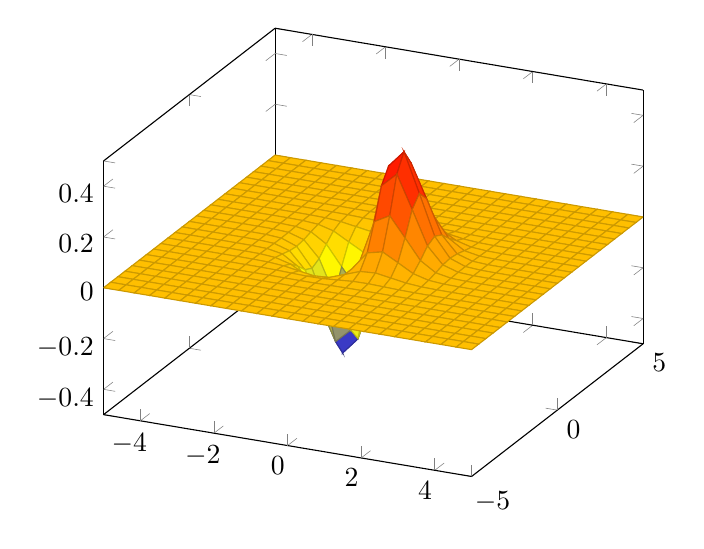
\begin{tikzpicture}
  \begin{axis}
  \addplot3[
      surf,
  ]
  {exp(-x^2-y^2)*x};
  \end{axis}
  \end{tikzpicture}
\end{figure}
\end{frame}
%%%%%%%%%%%%%%%%%%%%%%%%%%%%%%%%%%%%%%%%%%%%%%%%%

\begin{frame}
  \frametitle{tcbb}
  \centering
  \tcbb[0.5]{Fermat's Last Theorem}{
       Fermat's Last Theorem states that
       \[ x^n + y^n = z^n\]
       has no non-zero integer solutions for $x$, $y$ and $z$ when $n > 2$.
  }
\end{frame}

\begin{frame}\frametitle{block}
	\begin{block}{勾X定理:}
		直角三角形的斜边的平方等于两直角边的平方和。
		可以用符号语言表述为:设直角三角形ABC,其中$\angle C=90^\circ $则有
		\begin{equation}
			AB^2=BC^2+AC^2 \int
		\end{equation}
	\end{block}
	\begin{block}{Remark}
		Sample text
	\end{block}
\end{frame}

\begin{frame}
    \frametitle{alertblock}
	\begin{alertblock}{Important theorem}
		Sample text in red box
	\end{alertblock}
\end{frame}

\begin{frame}
    \frametitle{exampleblock}
	\begin{exampleblock} {Exampleblock}
		Sample text in green box. The title of the block is 'Examples'.
	\end{exampleblock}
    \begin{exampleblock} {例1:}
		Sample text in green box. The title of the block is 'Examples'.
	\end{exampleblock}
\end{frame}

\begin{frame}
    \frametitle{examples}
	\begin{examples}
		Sample text in green box. The title of the block is 'Examples'.
	\end{examples}
\end{frame}

\begin{frame}{tcolorbox}
  \begin{tcolorbox}[title=5.tcolorbox,colframe=red!75!black]
    This is tcolorbox
  \end{tcolorbox}
\end{frame}

\begin{frame}
    \frametitle{5.proof}
    \begin{proof}{证明:}
      {This is a proof}
    \end{proof}
\end{frame}

\begin{frame}
    \frametitle{自定义tcolorbox1$\to$4}
    \begin{tcolorbox1}[0.8]{tcolorbox1}
      This is tcolorbox1 that I defined
    \end{tcolorbox1}
    \begin{tcolorbox2}[0.86]{tcolorbox2}
      This is tcolorbox2 that I defined
    \end{tcolorbox2}
\end{frame}
\begin{frame}
  \frametitle{}
  \begin{tcolorbox3}[量子力学基本假设1/5]
    \lipsum[4]
  \end{tcolorbox3}
\end{frame}

\begin{frame}
    \begin{tcolorbox4}[量子力学基本假设1/5]
    \lipsum[4]
    \end{tcolorbox4}
\end{frame}

\begin{frame}
    \frametitle{tcbitemize}

    \tcbset{colback=white,arc=0mm,width = (\linewidth-4pt)/4,
    equal height group=AT,before=,after=\hfill,fonttitle=\bfseries}

    \noindent
    \foreach \n in {xxx,ggg,AAA,\"Agypten}
    {\begin{tcolorbox}[title=\n,colframe=red!75!black]
      Some content.
    \end{tcolorbox}}

    \noindent
    \foreach \n in {xxx,ggg,AAA,\"Agypten}
    {\begin{tcolorbox}[adjusted title=\n,colframe=blue!75!black]
    Some content.
    \end{tcolorbox}}

    \begin{tcbitemize}[raster columns=3,raster equal height,
              colframe=red!75!black,colback=red!5!white,fonttitle=\bfseries]
      \tcbitem[squeezed title={Short title}]
      First box
      \tcbitem[squeezed title={This is a very very long title}]
      Second box
      \tcbitem[squeezed title={This title is clearly to long for this application}] Third box
    \end{tcbitemize}
\end{frame}

\begin{frame}{选择题}

  一、单选题(每题2分)\\ \vspace{0.3em}
  1、下列说法正确的是: (\hspace{0.5em} )
  \xxxx{选项 A 的内容}{选项 B 的内容}{选项 C 的内容}{选项 D 的内容}
  2、下列说法正确的是: (\hspace{0.5em} )
  \xxxx{选项 A 的内容的内容的内容的内容的内容}{选项 B 的内容}{选项 C 的内容}{选项 D 的内容}
\end{frame}

\begin{frame}
  \frametitle{量子线路}
  \begin{figure}
    \centerline{
      \begin{tikzpicture}[thick]
      %
      % `operator' will only be used by Hadamard (H) gates here.
      % `phase' is used for controlled phase gates (dots).
      % `surround' is used for the background box.
      \tikzstyle{operator} = [draw,fill=white,minimum size=1.5em]
      \tikzstyle{phase} = [fill,shape=circle,minimum size=5pt,inner sep=0pt]
      %\tikzstyle{surround} = [fill=blue!10,thick,draw=black,rounded corners=2mm]
      %
      % Qubits
      \node at (0,0) (q1) {\rs{0}};
      \node at (0,-1) (q2) {\rs{0}};
      \node at (0,-2) (q3) {\rs{0}};
      %
      % Column 1
      \node[operator] (op11) at (1,0) {H} edge [-] (q1);
      \node[operator] (op21) at (1,-1) {H} edge [-] (q2);
      \node[operator] (op31) at (1,-2) {H} edge [-] (q3);
      %
      % Column 3
      \node[phase] (phase11) at (2,0) {} edge [-] (op11);
      \node[phase] (phase12) at (2,-1) {} edge [-] (op21);
      \draw[-] (phase11) -- (phase12);
      %
      % Column 4
      \node[phase] (phase21) at (3,0) {} edge [-] (phase11);
      \node[phase] (phase23) at (3,-2) {} edge [-] (op31);
      \draw[-] (phase21) -- (phase23);
      %
      % Column 5
      \node[operator] (op24) at (4,-1) {H} edge [-] (phase12);
      \node[operator] (op34) at (4,-2) {H} edge [-] (phase23);
      %
      % Column 6
      \node (end1) at (5,0) {} edge [-] (phase21);
      \node (end2) at (5,-1) {} edge [-] (op24);
      \node (end3) at (5,-2) {} edge [-] (op34);
      %
      % Bracket
      \draw[decorate,decoration={brace},thick] (5,0.2) to
    node[midway,right] (bracket) {$\dfrac{\rs{000}+\rs{111}}{\sqrt{2}}$}
    (5,-2.2);
      %
      % Background Box
      %\begin{pgfonlayer}{background}
      %\node[surround] (background) [fit = (q1) (op31) (bracket)] {};
      %\end{pgfonlayer}
      %
      \end{tikzpicture}
    }
    \caption{
      A quantum circuit for producing a GHZ state using
      Hadamard gates and controlled phase gates.
    }
  \end{figure}
\end{frame}

\begin{frame}
  \frametitle{}
  \centering
  \begin{tikzpicture}

    % define coordinates
    \coordinate (O) at (0,0) ;
    \coordinate (A) at (0,4) ;
    \coordinate (B) at (0,-4) ;

    % media
    \fill[blue!25!,opacity=.3] (-4,0) rectangle (4,4);
    \fill[blue!60!,opacity=.3] (-4,0) rectangle (4,-4);
    \node[right] at (2,2) {Air};
    \node[left] at (-2,-2) {Water};

    % axis
    \draw[dash pattern=on5pt off3pt] (A) -- (B) ;

    % rays
    \draw[red,ultra thick,reverse directed] (O) -- (130:5.2);
    \draw[blue,directed,ultra thick] (O) -- (-70:4.24);

    % angles
    \draw (0,1) arc (90:130:1);
    \draw (0,-1.4) arc (270:290:1.4) ;
    \node[] at (280:1.8)  {$\theta_{2}$};
    \node[] at (110:1.4)  {$\theta_{1}$};
\end{tikzpicture}
\end{frame}

\begin{frame}
  \frametitle{Intersecting lines}
  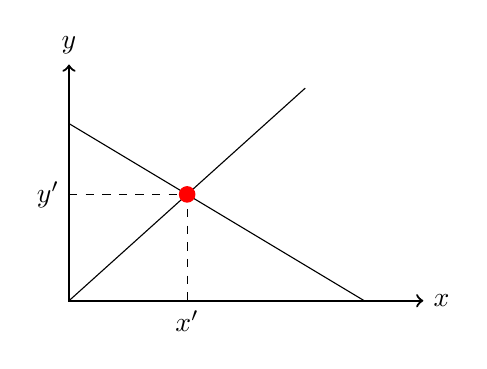
\begin{tikzpicture}[scale=1.5]
    % Draw axes
    \draw [<->,thick] (0,2) node (yaxis) [above] {$y$}
        |- (3,0) node (xaxis) [right] {$x$};
    % Draw two intersecting lines
    \draw (0,0) coordinate (a_1) -- (2,1.8) coordinate (a_2);
    \draw (0,1.5) coordinate (b_1) -- (2.5,0) coordinate (b_2);
    % Calculate the intersection of the lines a_1 -- a_2 and b_1 -- b_2
    % and store the coordinate in c.
    \coordinate (c) at (intersection of a_1--a_2 and b_1--b_2);
    % Draw lines indicating intersection with y and x axis. Here we use
    % the perpendicular coordinate system
    \draw[dashed] (yaxis |- c) node[left] {$y'$}
        -| (xaxis -| c) node[below] {$x'$};
    % Draw a dot to indicate intersection point
    \fill[red] (c) circle (2pt);
\end{tikzpicture}
\end{frame}

\begin{frame}
  \frametitle{Rigid body dynamics}
  \tikzstyle{na} = [baseline=-.5ex]
  % Below we mix an ordinary equation with TikZ nodes defined by Myitem. Note that we have to
  % adjust the baseline of the nodes to get proper alignment with the rest of
  % the equation.
  \begin{equation*}
  \vec{a}_p = \vec{a}_o+\frac{{}^b d^2}{dt^2}\vec{r} +
          \Myitem{t1}{blue}{2\vec{\omega}_{ib}\times\frac{{}^b d}{dt}\vec{r}}
          +
          \Myitem{t2}{red}{\vec{\alpha}_{ib}\times\vec{r}}
          +
          \Myitem{t3}{green}{\vec{\omega}_{ib}\times(\vec{\omega}_{ib}\times\vec{r})}
  \end{equation*}
  \begin{itemize}[<+-| alert@+>]
    \item Coriolis acceleration
        \tikz[na] \node[coordinate] (n1) {};
    \item Transversal acceleration
        \tikz[na]\node [coordinate] (n2) {};
    \item Centripetal acceleration
        \tikz[na]\node [coordinate] (n3) {};
  \end{itemize}
  % Now it's time to draw some edges between the global nodes. Note that we
  % have to apply the 'overlay' style.
  \begin{tikzpicture}[overlay]
          \path[->]<1-> (n1) edge [bend right] (t1);
          \path[->]<2-> (n2) edge [bend right] (t2);
          \path[->]<3-> (n3) edge [out=0, in=-90] (t3);
  \end{tikzpicture}
\end{frame}

\begin{frame}{Make Titles Informative.}

  You can create overlays\dots
  \begin{itemize}
  \item using the \texttt{pause} command:
    \begin{itemize}
    \item
      First item.
      \pause
    \item
      Second item.
    \end{itemize}
  \item
    using overlay specifications:
    \begin{itemize}
    \item<3->
      First item.
    \item<4->
      Second item.
    \end{itemize}
  \item
    using the general \texttt{uncover} command:
    \begin{itemize}
      \uncover<5->{\item
        First item.}
      \uncover<6->{\item
        Second item.}
    \end{itemize}
  \end{itemize}
\end{frame}

\begin{frame}
  \frametitle{}

  \begin{center} %Optional, but helps to tidy up the layout
  \begin{tikzpicture}[scale=.1] %Scale must be changed to make the flag fit on letter/A4 paper (scale=1 produces a 30 cm by 20 cm flag)
  \clip (-15,-10) rectangle (15,10); %Optional, crops the flag to the correct size
  \draw[black] (-15,-10)--(15,-10)--(15,10)--(-15,10)--cycle; %Optional, draws a border around the flag
  \fill[chred] (-15,-10)--(15,-10)--(15,10)--(-15,10)--cycle; %Red background

  %Template for a star, this can be shifted, scaled and rotated as you wish
  \def\star{(0,4)--({sqrt(50-22*sqrt(5))},{-1+sqrt(5)})--({+sqrt(10+2*sqrt(5))},{-1+sqrt(5)})--({2*sqrt(5-2*sqrt(5))},{+4-2*sqrt(5)})--({+sqrt(10-2*sqrt(5))},{-1-sqrt(5)})--(0,{-6+2*sqrt(5)})--({-sqrt(10-2*sqrt(5))},{-1-sqrt(5)})--({-2*sqrt(5-2*sqrt(5))},{+4-2*sqrt(5)})--({-sqrt(10+2*sqrt(5))},{-1+sqrt(5)})--({-sqrt(50-22*sqrt(5))},{-1+sqrt(5)})--cycle}

  %Outer scope for shifting, scaling and rotation of the entire 5-star pattern
  \begin{scope}[shift={(-10,5)},scale=1,rotate=0]
  %Inner scopes for shifting, scaling and rotation of each individual star
  \begin{scope}[shift={(0,0)},scale=3/4,rotate=0]
  \fill[chyel] \star; %Large star
  \end{scope}
  %Small stars, clockwise from the top
  \begin{scope}[shift={(5,3)},scale=1/4,rotate=90+atan(3/5)]
  \fill[chyel] \star;
  \end{scope}
  \begin{scope}[shift={(7,1)},scale=1/4,rotate=90+atan(1/7)]
  \fill[chyel] \star;
  \end{scope}
  \begin{scope}[shift={(7,-2)},scale=1/4,rotate=90-atan(2/7)]
  \fill[chyel] \star;
  \end{scope}
  \begin{scope}[shift={(5,-4)},scale=1/4,rotate=90-atan(4/5)]
  \fill[chyel] \star;
  \end{scope}
  \end{scope}
  \end{tikzpicture}
  \end{center}
\end{frame}

\begin{frame}
    \frametitle{}
    \tcbset{enhanced jigsaw,fonttitle=\bfseries,opacityback=0.35,colback=blue!5!white,
        frame style={left color=red!75!black,right color=red!10!yellow}}
    
\begin{tikzpicture}% draw two balls
      \path[use as bounding box] (0,0.8) rectangle +(0.1,0.1);
      \shadedraw [shading=ball] (0,0.3) circle (1cm);
      %\shadedraw [ball color=yellow!20] (3,-2.2) circle (1cm);
    \end{tikzpicture}
    \begin{tcolorbox}[title=\faEnvira\hspace{1em} 结论,
      overlay=
      {\begin{tcbinvclipframe}
      \draw[red,line width=1cm] ([xshift=-2mm,yshift=2mm]frame.north west)
      --([xshift=2mm,yshift=-2mm]frame.south east);
      \draw[red,line width=1cm] ([xshift=-2mm,yshift=-2mm]frame.south west)
      --([xshift=2mm,yshift=2mm]frame.north east);
      \end{tcbinvclipframe}}]
      \lipsum[2]
      \end{tcolorbox}
\end{frame}
